% Overview of the spatially-homogeneous two-temperature relaxation benchmark.
% Standalone: % Overview of the spatially-homogeneous two-temperature relaxation benchmark.
% Standalone: % Overview of the spatially-homogeneous two-temperature relaxation benchmark.
% Standalone: % Overview of the spatially-homogeneous two-temperature relaxation benchmark.
% Standalone: \input{benchmark_temperature_relaxation} from main.tex.
% Requires graphicx; figures live in figures/fig_polyrelax_*.pdf.
% Produced by benchmark_polyatomic_temperature_relaxation.m.
\section{Spatially-homogeneous two-temperature relaxation}
\label{sec:relax}

As a fully nonlinear, time-dependent check of the DSMC operator we relax a $0$D (space-homogeneous)
gas from a genuine product of Maxwellians, $f(\vv,I,0)=M_{\vv}(T_v^0)\,M_I(T_I^0)$ with the
translational temperature $T_v^0$ and internal temperature $T_I^0$ deliberately unequal. The
distribution is projected onto the spectral basis by tensor-product Gauss--Laguerre quadrature and
advanced with an explicit RK2 (Heun) integrator of the quadratic operator $Q(\bm{c},\bm{c})$. This
exercises the operator's core physical task -- exchanging energy between the translational and
internal degrees of freedom -- while the invariants are held fixed, and it is the polyatomic
counterpart of the classical Bobylev--Krook--Wu relaxation.

In reduced units (equilibrium reference $T=1$, internal degrees of freedom $d_i=\delta$) energy
conservation fixes the common equilibrium temperature to
\begin{equation}
  T_{\mathrm{eq}}=\frac{3\,T_v^0+d_i\,T_I^0}{3+d_i},
  \qquad
  E=\tfrac32 T_v+\tfrac{\delta}{2}T_I=\text{const}.
  \label{eq:Teq}
\end{equation}
The two temperatures are read off exactly as linear moment functionals of the coefficient vector
($T_v=\langle|\vv|^2\rangle/3$, $T_I=\langle I\rangle/(\nu+1)$), so they remain exact regardless of
basis truncation. Two sweeps isolate the two independent controls (all runs use
$K_{\max}=I_{\max}=2$, $L_{\max}=2$, $T_v^0=1.4$, $T_I^0=1.0$, $\zeta=0.5$):

\begin{itemize}
\item \textbf{Internal degrees of freedom $d_i$} (Fig.~\ref{fig:relax_di}, $\omega=1$). The same
initial state relaxes to a \emph{different} $T_{\mathrm{eq}}$ for each $d_i\in\{2,4,6\}$; the
numerical late-time value reproduces \eqref{eq:Teq} to four digits ($1.2400,\ 1.1714,\ 1.1333$).
\item \textbf{DSMC convex-split weight $\omega$} (Fig.~\ref{fig:relax_omega}, $d_i=2$). Because
energy conservation is independent of $\omega$, every $\omega$ relaxes to the \emph{same}
$T_{\mathrm{eq}}=1.240$, but at a \emph{different} rate. The frozen channel is elastic and leaves
both energy modes $(1,0,0)$ and $(0,1,0)$ invariant, so its energy-exchange block vanishes and the
$T_v-T_I$ relaxation rate is exactly proportional to $\omega$: the measured slopes yield
$r(\omega)/r(1)=0.251,\,0.502,\,0.751,\,1.000$.
\end{itemize}

Throughout the relaxation the state stays isotropic (all $l\ge1$ amplitudes remain at $0$ to
machine precision, so momentum is trivially conserved), and the total energy \eqref{eq:Teq} is
conserved to $\sim3\times10^{-12}$ while its translational and internal parts each change by tens of
percent (Fig.~\ref{fig:relax_cons}); the mass row is pinned at the round-off floor.

\begin{figure}[t]
\centering
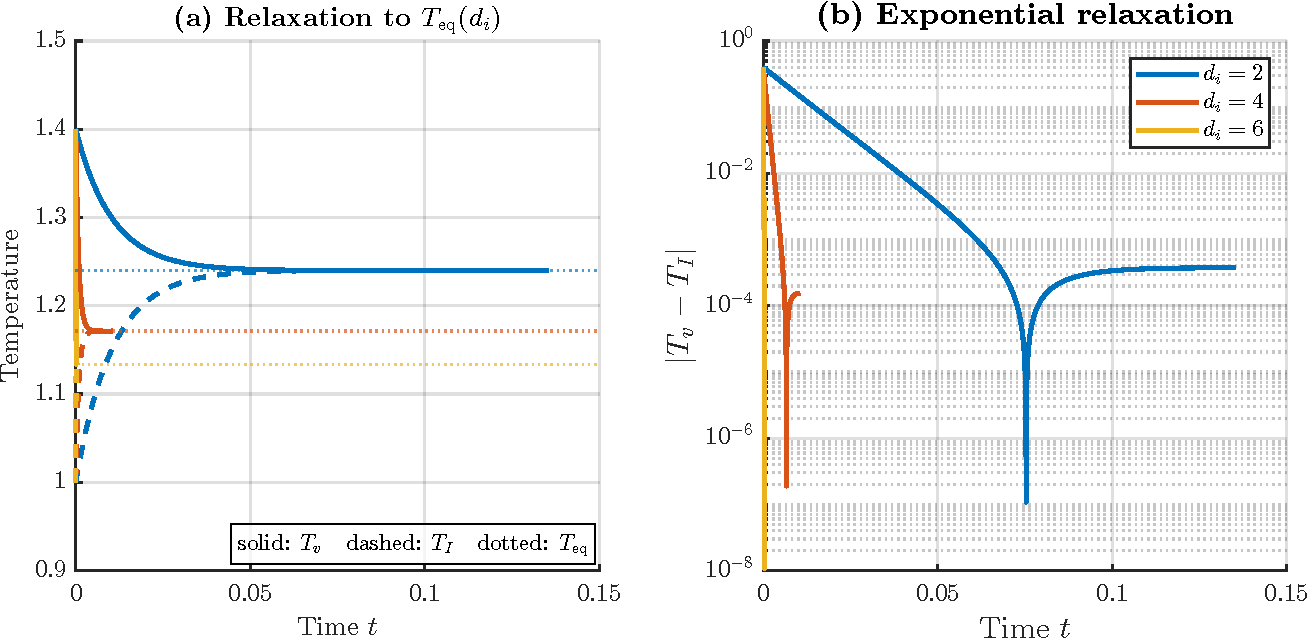
\includegraphics[width=0.9\textwidth]{figures/fig_polyrelax_sweep_di.pdf}
\caption{Relaxation for varying internal degrees of freedom $d_i$ ($\omega=1$). (a) $T_v$ (solid)
and $T_I$ (dashed) converge to the predicted $T_{\mathrm{eq}}(d_i)$ of \eqref{eq:Teq} (dotted).
(b) The temperature difference $|T_v-T_I|$ decays exponentially; larger $d_i$ relaxes faster.}
\label{fig:relax_di}
\end{figure}

\begin{figure}[t]
\centering
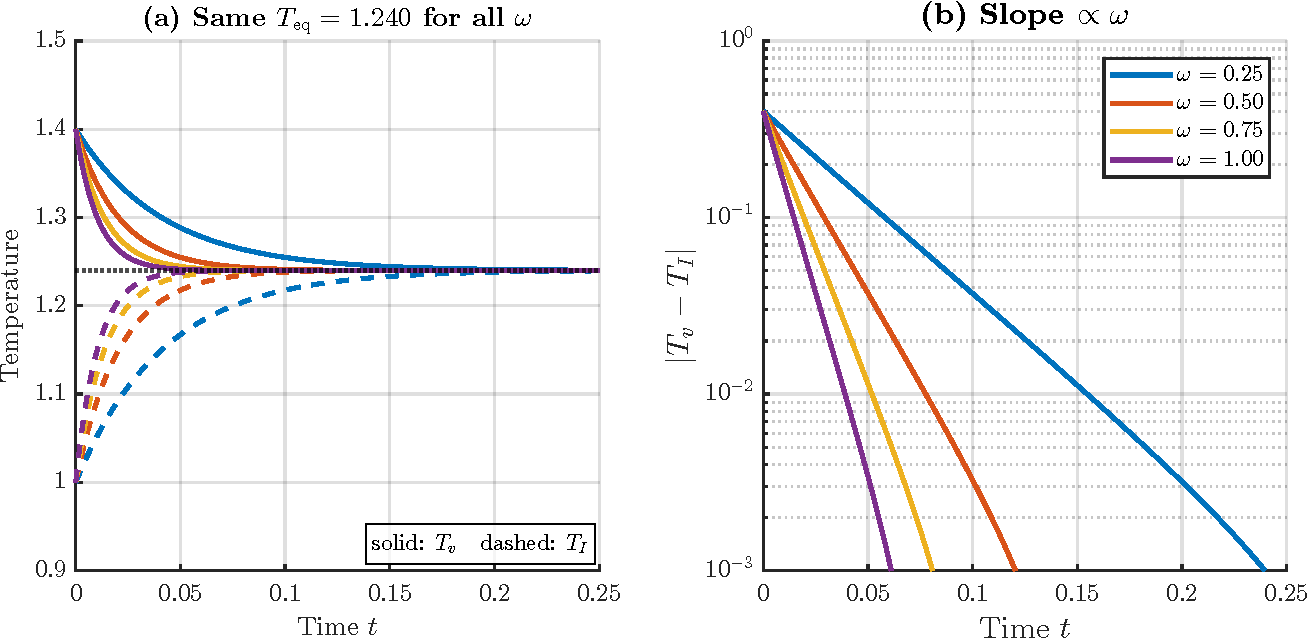
\includegraphics[width=0.9\textwidth]{figures/fig_polyrelax_sweep_omega.pdf}
\caption{Relaxation for varying DSMC weight $\omega$ at fixed $d_i=2$. (a) All $\omega$ reach the
same $T_{\mathrm{eq}}=1.240$. (b) The semilog decay of $|T_v-T_I|$ has slope proportional to
$\omega$ (measured rate $r$ in the legend), a direct consequence of the frozen channel being
elastic.}
\label{fig:relax_omega}
\end{figure}

\begin{figure}[t]
\centering
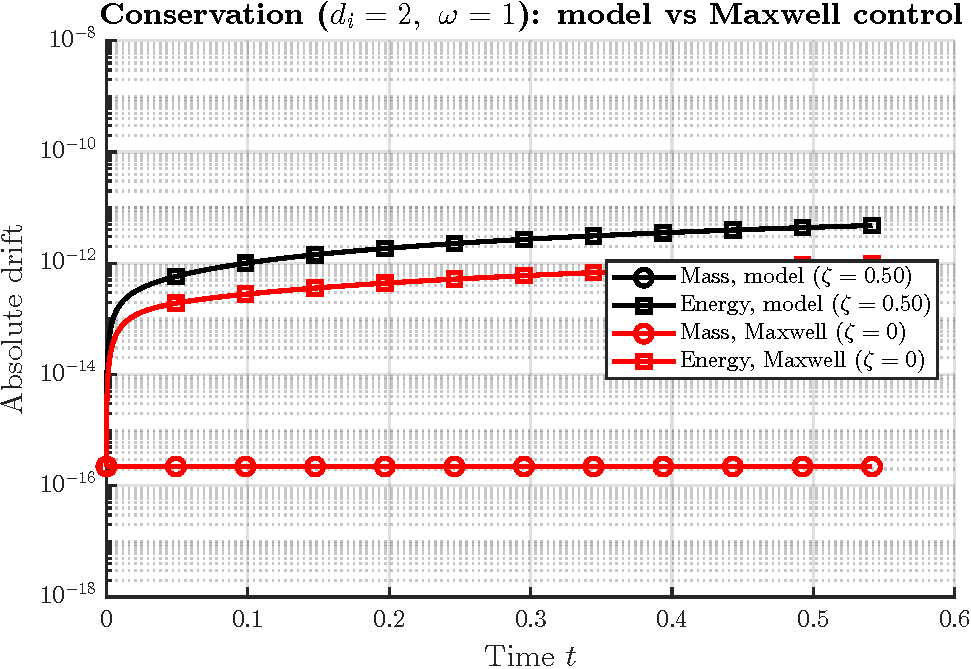
\includegraphics[width=0.62\textwidth]{figures/fig_polyrelax_conservation.pdf}
\caption{Conservation during the $d_i=2,\ \omega=1$ run. Total energy drifts by only
$\sim3\times10^{-12}$ (RK2 accumulation) and the mass row sits at the round-off floor, even though
$T_v$ and $T_I$ individually vary substantially.}
\label{fig:relax_cons}
\end{figure}
 from main.tex.
% Requires graphicx; figures live in figures/fig_polyrelax_*.pdf.
% Produced by benchmark_polyatomic_temperature_relaxation.m.
\section{Spatially-homogeneous two-temperature relaxation}
\label{sec:relax}

As a fully nonlinear, time-dependent check of the DSMC operator we relax a $0$D (space-homogeneous)
gas from a genuine product of Maxwellians, $f(\vv,I,0)=M_{\vv}(T_v^0)\,M_I(T_I^0)$ with the
translational temperature $T_v^0$ and internal temperature $T_I^0$ deliberately unequal. The
distribution is projected onto the spectral basis by tensor-product Gauss--Laguerre quadrature and
advanced with an explicit RK2 (Heun) integrator of the quadratic operator $Q(\bm{c},\bm{c})$. This
exercises the operator's core physical task -- exchanging energy between the translational and
internal degrees of freedom -- while the invariants are held fixed, and it is the polyatomic
counterpart of the classical Bobylev--Krook--Wu relaxation.

In reduced units (equilibrium reference $T=1$, internal degrees of freedom $d_i=\delta$) energy
conservation fixes the common equilibrium temperature to
\begin{equation}
  T_{\mathrm{eq}}=\frac{3\,T_v^0+d_i\,T_I^0}{3+d_i},
  \qquad
  E=\tfrac32 T_v+\tfrac{\delta}{2}T_I=\text{const}.
  \label{eq:Teq}
\end{equation}
The two temperatures are read off exactly as linear moment functionals of the coefficient vector
($T_v=\langle|\vv|^2\rangle/3$, $T_I=\langle I\rangle/(\nu+1)$), so they remain exact regardless of
basis truncation. Two sweeps isolate the two independent controls (all runs use
$K_{\max}=I_{\max}=2$, $L_{\max}=2$, $T_v^0=1.4$, $T_I^0=1.0$, $\zeta=0.5$):

\begin{itemize}
\item \textbf{Internal degrees of freedom $d_i$} (Fig.~\ref{fig:relax_di}, $\omega=1$). The same
initial state relaxes to a \emph{different} $T_{\mathrm{eq}}$ for each $d_i\in\{2,4,6\}$; the
numerical late-time value reproduces \eqref{eq:Teq} to four digits ($1.2400,\ 1.1714,\ 1.1333$).
\item \textbf{DSMC convex-split weight $\omega$} (Fig.~\ref{fig:relax_omega}, $d_i=2$). Because
energy conservation is independent of $\omega$, every $\omega$ relaxes to the \emph{same}
$T_{\mathrm{eq}}=1.240$, but at a \emph{different} rate. The frozen channel is elastic and leaves
both energy modes $(1,0,0)$ and $(0,1,0)$ invariant, so its energy-exchange block vanishes and the
$T_v-T_I$ relaxation rate is exactly proportional to $\omega$: the measured slopes yield
$r(\omega)/r(1)=0.251,\,0.502,\,0.751,\,1.000$.
\end{itemize}

Throughout the relaxation the state stays isotropic (all $l\ge1$ amplitudes remain at $0$ to
machine precision, so momentum is trivially conserved), and the total energy \eqref{eq:Teq} is
conserved to $\sim3\times10^{-12}$ while its translational and internal parts each change by tens of
percent (Fig.~\ref{fig:relax_cons}); the mass row is pinned at the round-off floor.

\begin{figure}[t]
\centering
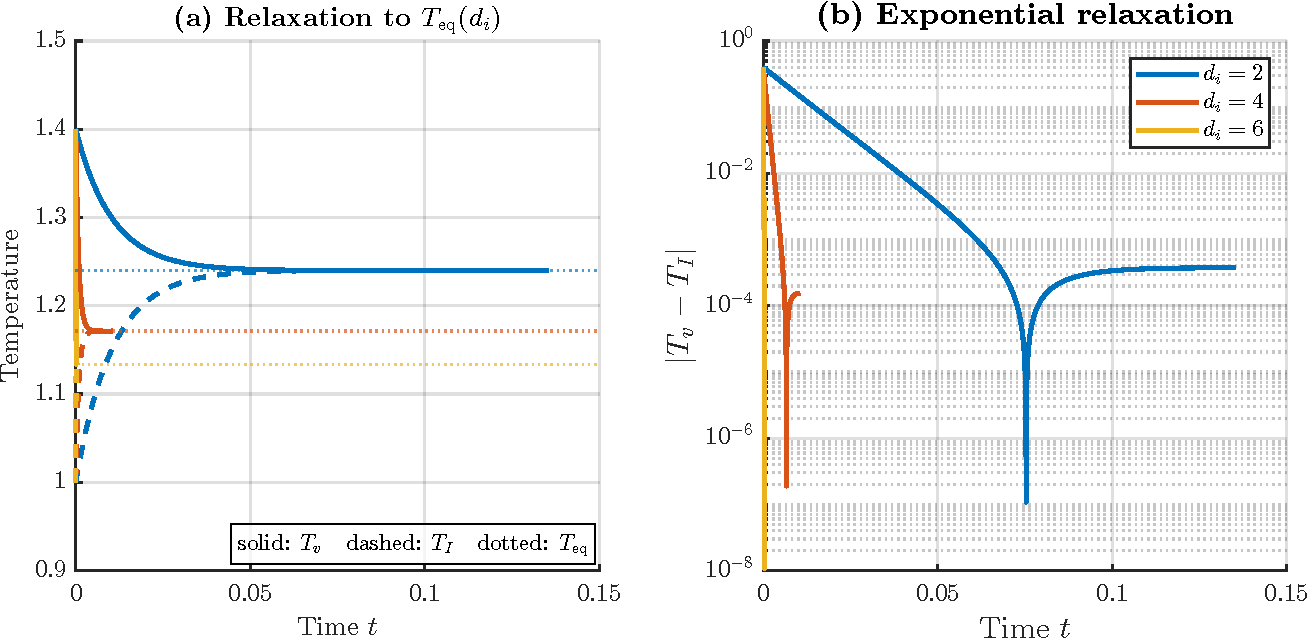
\includegraphics[width=0.9\textwidth]{figures/fig_polyrelax_sweep_di.pdf}
\caption{Relaxation for varying internal degrees of freedom $d_i$ ($\omega=1$). (a) $T_v$ (solid)
and $T_I$ (dashed) converge to the predicted $T_{\mathrm{eq}}(d_i)$ of \eqref{eq:Teq} (dotted).
(b) The temperature difference $|T_v-T_I|$ decays exponentially; larger $d_i$ relaxes faster.}
\label{fig:relax_di}
\end{figure}

\begin{figure}[t]
\centering
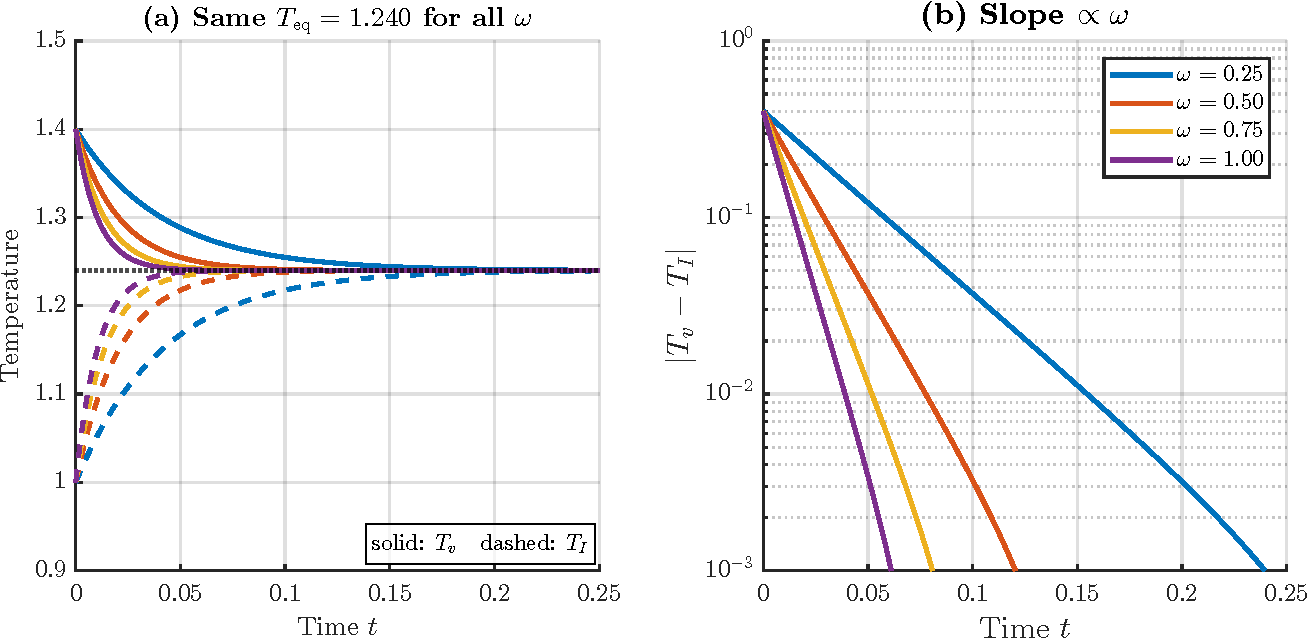
\includegraphics[width=0.9\textwidth]{figures/fig_polyrelax_sweep_omega.pdf}
\caption{Relaxation for varying DSMC weight $\omega$ at fixed $d_i=2$. (a) All $\omega$ reach the
same $T_{\mathrm{eq}}=1.240$. (b) The semilog decay of $|T_v-T_I|$ has slope proportional to
$\omega$ (measured rate $r$ in the legend), a direct consequence of the frozen channel being
elastic.}
\label{fig:relax_omega}
\end{figure}

\begin{figure}[t]
\centering
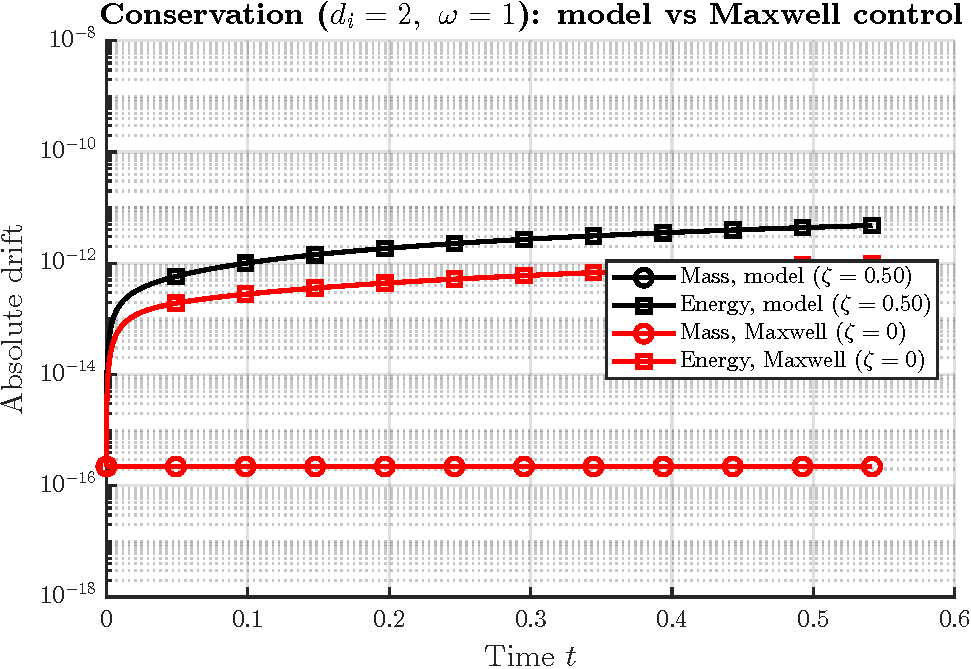
\includegraphics[width=0.62\textwidth]{figures/fig_polyrelax_conservation.pdf}
\caption{Conservation during the $d_i=2,\ \omega=1$ run. Total energy drifts by only
$\sim3\times10^{-12}$ (RK2 accumulation) and the mass row sits at the round-off floor, even though
$T_v$ and $T_I$ individually vary substantially.}
\label{fig:relax_cons}
\end{figure}
 from main.tex.
% Requires graphicx; figures live in figures/fig_polyrelax_*.pdf.
% Produced by benchmark_polyatomic_temperature_relaxation.m.
\section{Spatially-homogeneous two-temperature relaxation}
\label{sec:relax}

As a fully nonlinear, time-dependent check of the DSMC operator we relax a $0$D (space-homogeneous)
gas from a genuine product of Maxwellians, $f(\vv,I,0)=M_{\vv}(T_v^0)\,M_I(T_I^0)$ with the
translational temperature $T_v^0$ and internal temperature $T_I^0$ deliberately unequal. The
distribution is projected onto the spectral basis by tensor-product Gauss--Laguerre quadrature and
advanced with an explicit RK2 (Heun) integrator of the quadratic operator $Q(\bm{c},\bm{c})$. This
exercises the operator's core physical task -- exchanging energy between the translational and
internal degrees of freedom -- while the invariants are held fixed, and it is the polyatomic
counterpart of the classical Bobylev--Krook--Wu relaxation.

In reduced units (equilibrium reference $T=1$, internal degrees of freedom $d_i=\delta$) energy
conservation fixes the common equilibrium temperature to
\begin{equation}
  T_{\mathrm{eq}}=\frac{3\,T_v^0+d_i\,T_I^0}{3+d_i},
  \qquad
  E=\tfrac32 T_v+\tfrac{\delta}{2}T_I=\text{const}.
  \label{eq:Teq}
\end{equation}
The two temperatures are read off exactly as linear moment functionals of the coefficient vector
($T_v=\langle|\vv|^2\rangle/3$, $T_I=\langle I\rangle/(\nu+1)$), so they remain exact regardless of
basis truncation. Two sweeps isolate the two independent controls (all runs use
$K_{\max}=I_{\max}=2$, $L_{\max}=2$, $T_v^0=1.4$, $T_I^0=1.0$, $\zeta=0.5$):

\begin{itemize}
\item \textbf{Internal degrees of freedom $d_i$} (Fig.~\ref{fig:relax_di}, $\omega=1$). The same
initial state relaxes to a \emph{different} $T_{\mathrm{eq}}$ for each $d_i\in\{2,4,6\}$; the
numerical late-time value reproduces \eqref{eq:Teq} to four digits ($1.2400,\ 1.1714,\ 1.1333$).
\item \textbf{DSMC convex-split weight $\omega$} (Fig.~\ref{fig:relax_omega}, $d_i=2$). Because
energy conservation is independent of $\omega$, every $\omega$ relaxes to the \emph{same}
$T_{\mathrm{eq}}=1.240$, but at a \emph{different} rate. The frozen channel is elastic and leaves
both energy modes $(1,0,0)$ and $(0,1,0)$ invariant, so its energy-exchange block vanishes and the
$T_v-T_I$ relaxation rate is exactly proportional to $\omega$: the measured slopes yield
$r(\omega)/r(1)=0.251,\,0.502,\,0.751,\,1.000$.
\end{itemize}

Throughout the relaxation the state stays isotropic (all $l\ge1$ amplitudes remain at $0$ to
machine precision, so momentum is trivially conserved), and the total energy \eqref{eq:Teq} is
conserved to $\sim3\times10^{-12}$ while its translational and internal parts each change by tens of
percent (Fig.~\ref{fig:relax_cons}); the mass row is pinned at the round-off floor.

\begin{figure}[t]
\centering
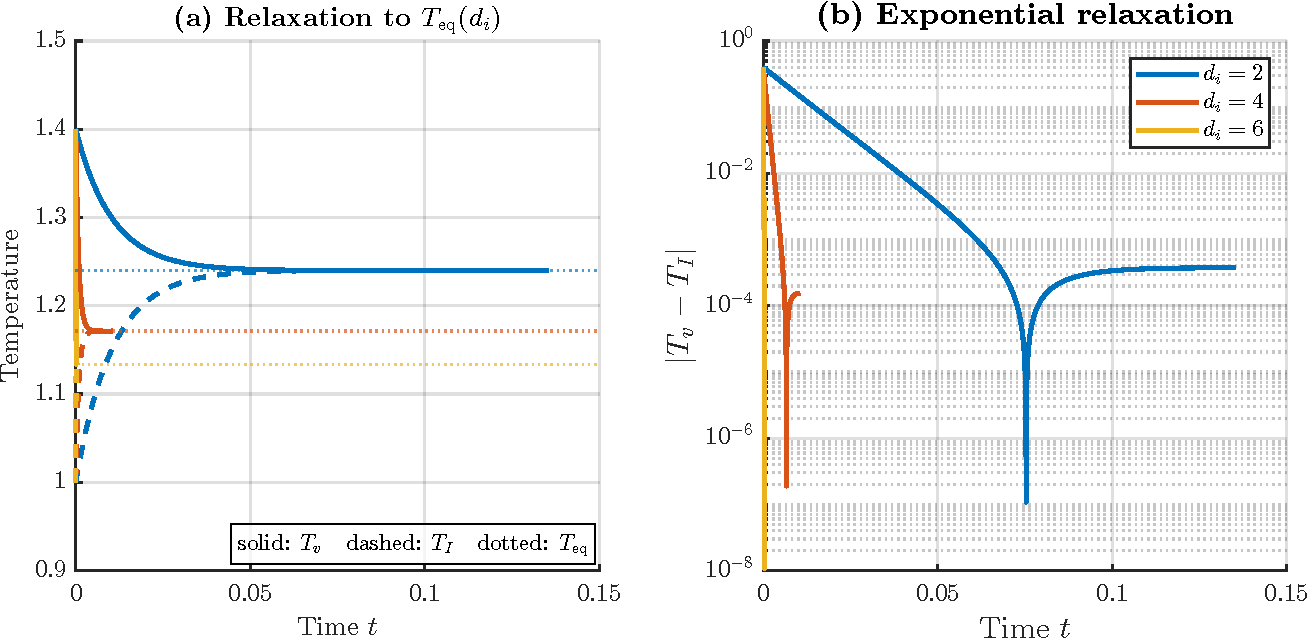
\includegraphics[width=0.9\textwidth]{figures/fig_polyrelax_sweep_di.pdf}
\caption{Relaxation for varying internal degrees of freedom $d_i$ ($\omega=1$). (a) $T_v$ (solid)
and $T_I$ (dashed) converge to the predicted $T_{\mathrm{eq}}(d_i)$ of \eqref{eq:Teq} (dotted).
(b) The temperature difference $|T_v-T_I|$ decays exponentially; larger $d_i$ relaxes faster.}
\label{fig:relax_di}
\end{figure}

\begin{figure}[t]
\centering
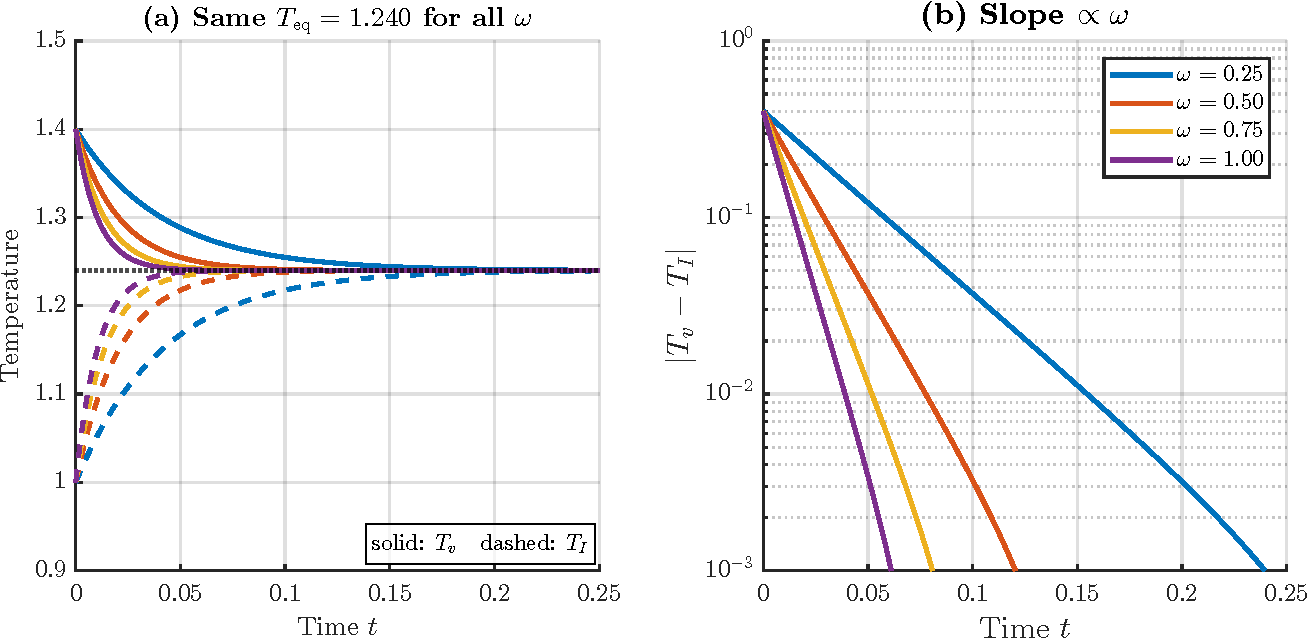
\includegraphics[width=0.9\textwidth]{figures/fig_polyrelax_sweep_omega.pdf}
\caption{Relaxation for varying DSMC weight $\omega$ at fixed $d_i=2$. (a) All $\omega$ reach the
same $T_{\mathrm{eq}}=1.240$. (b) The semilog decay of $|T_v-T_I|$ has slope proportional to
$\omega$ (measured rate $r$ in the legend), a direct consequence of the frozen channel being
elastic.}
\label{fig:relax_omega}
\end{figure}

\begin{figure}[t]
\centering
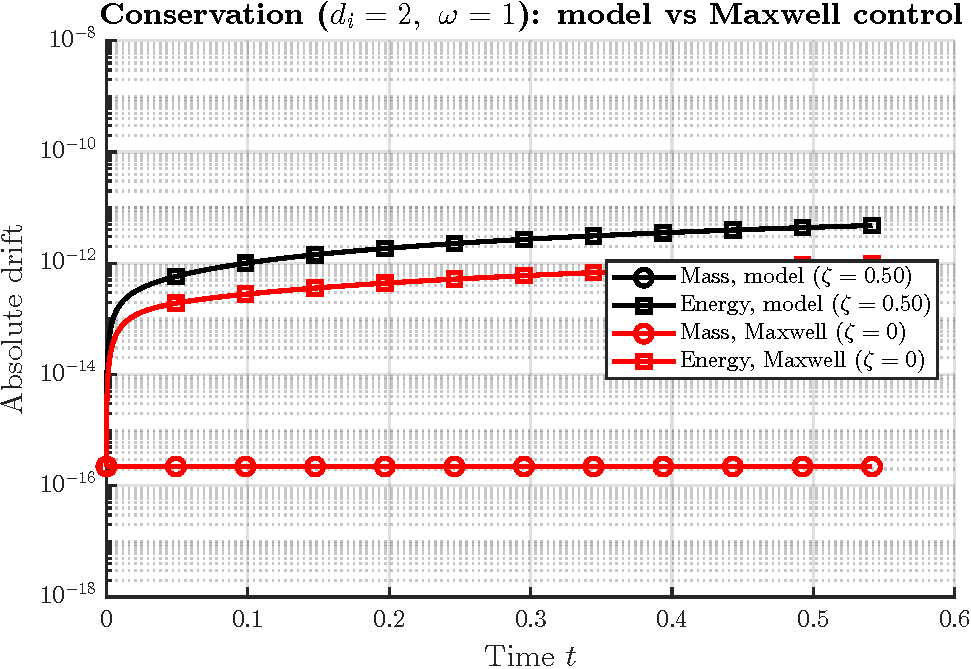
\includegraphics[width=0.62\textwidth]{figures/fig_polyrelax_conservation.pdf}
\caption{Conservation during the $d_i=2,\ \omega=1$ run. Total energy drifts by only
$\sim3\times10^{-12}$ (RK2 accumulation) and the mass row sits at the round-off floor, even though
$T_v$ and $T_I$ individually vary substantially.}
\label{fig:relax_cons}
\end{figure}
 from main.tex.
% Requires graphicx; figures live in figures/fig_polyrelax_*.pdf.
% Produced by benchmark_polyatomic_temperature_relaxation.m.
\section{Spatially-homogeneous two-temperature relaxation}
\label{sec:relax}

As a fully nonlinear, time-dependent check of the DSMC operator we relax a $0$D (space-homogeneous)
gas from a genuine product of Maxwellians, $f(\vv,I,0)=M_{\vv}(T_v^0)\,M_I(T_I^0)$ with the
translational temperature $T_v^0$ and internal temperature $T_I^0$ deliberately unequal. The
distribution is projected onto the spectral basis by tensor-product Gauss--Laguerre quadrature and
advanced with an explicit RK2 (Heun) integrator of the quadratic operator $Q(\bm{c},\bm{c})$. This
exercises the operator's core physical task -- exchanging energy between the translational and
internal degrees of freedom -- while the invariants are held fixed, and it is the polyatomic
counterpart of the classical Bobylev--Krook--Wu relaxation.

In reduced units (equilibrium reference $T=1$, internal degrees of freedom $d_i=\delta$) energy
conservation fixes the common equilibrium temperature to
\begin{equation}
  T_{\mathrm{eq}}=\frac{3\,T_v^0+d_i\,T_I^0}{3+d_i},
  \qquad
  E=\tfrac32 T_v+\tfrac{\delta}{2}T_I=\text{const}.
  \label{eq:Teq}
\end{equation}
The two temperatures are read off exactly as linear moment functionals of the coefficient vector
($T_v=\langle|\vv|^2\rangle/3$, $T_I=\langle I\rangle/(\nu+1)$), so they remain exact regardless of
basis truncation. Two sweeps isolate the two independent controls (all runs use
$K_{\max}=I_{\max}=2$, $L_{\max}=2$, $T_v^0=1.4$, $T_I^0=1.0$, $\zeta=0.5$):

\begin{itemize}
\item \textbf{Internal degrees of freedom $d_i$} (Fig.~\ref{fig:relax_di}, $\omega=1$). The same
initial state relaxes to a \emph{different} $T_{\mathrm{eq}}$ for each $d_i\in\{2,4,6\}$; the
numerical late-time value reproduces \eqref{eq:Teq} to four digits ($1.2400,\ 1.1714,\ 1.1333$).
\item \textbf{DSMC convex-split weight $\omega$} (Fig.~\ref{fig:relax_omega}, $d_i=2$). Because
energy conservation is independent of $\omega$, every $\omega$ relaxes to the \emph{same}
$T_{\mathrm{eq}}=1.240$, but at a \emph{different} rate. The frozen channel is elastic and leaves
both energy modes $(1,0,0)$ and $(0,1,0)$ invariant, so its energy-exchange block vanishes and the
$T_v-T_I$ relaxation rate is exactly proportional to $\omega$: the measured slopes yield
$r(\omega)/r(1)=0.251,\,0.502,\,0.751,\,1.000$.
\end{itemize}

Throughout the relaxation the state stays isotropic (all $l\ge1$ amplitudes remain at $0$ to
machine precision, so momentum is trivially conserved), and the total energy \eqref{eq:Teq} is
conserved to $\sim3\times10^{-12}$ while its translational and internal parts each change by tens of
percent (Fig.~\ref{fig:relax_cons}); the mass row is pinned at the round-off floor.

\begin{figure}[t]
\centering
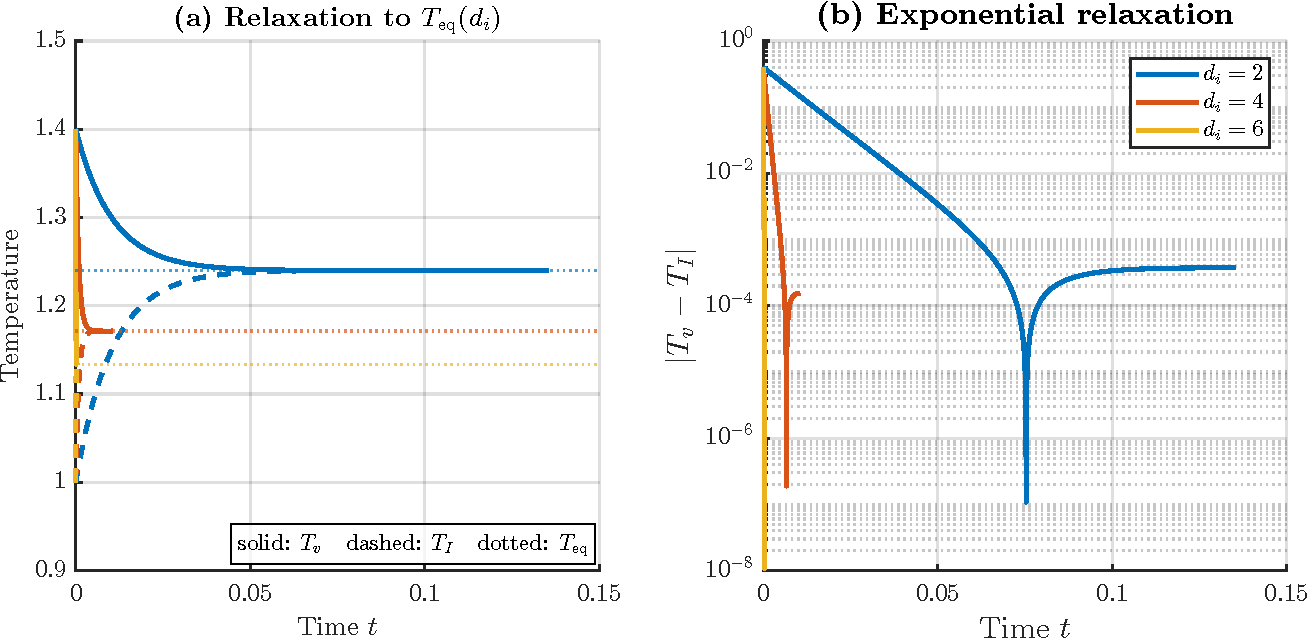
\includegraphics[width=0.9\textwidth]{figures/fig_polyrelax_sweep_di.pdf}
\caption{Relaxation for varying internal degrees of freedom $d_i$ ($\omega=1$). (a) $T_v$ (solid)
and $T_I$ (dashed) converge to the predicted $T_{\mathrm{eq}}(d_i)$ of \eqref{eq:Teq} (dotted).
(b) The temperature difference $|T_v-T_I|$ decays exponentially; larger $d_i$ relaxes faster.}
\label{fig:relax_di}
\end{figure}

\begin{figure}[t]
\centering
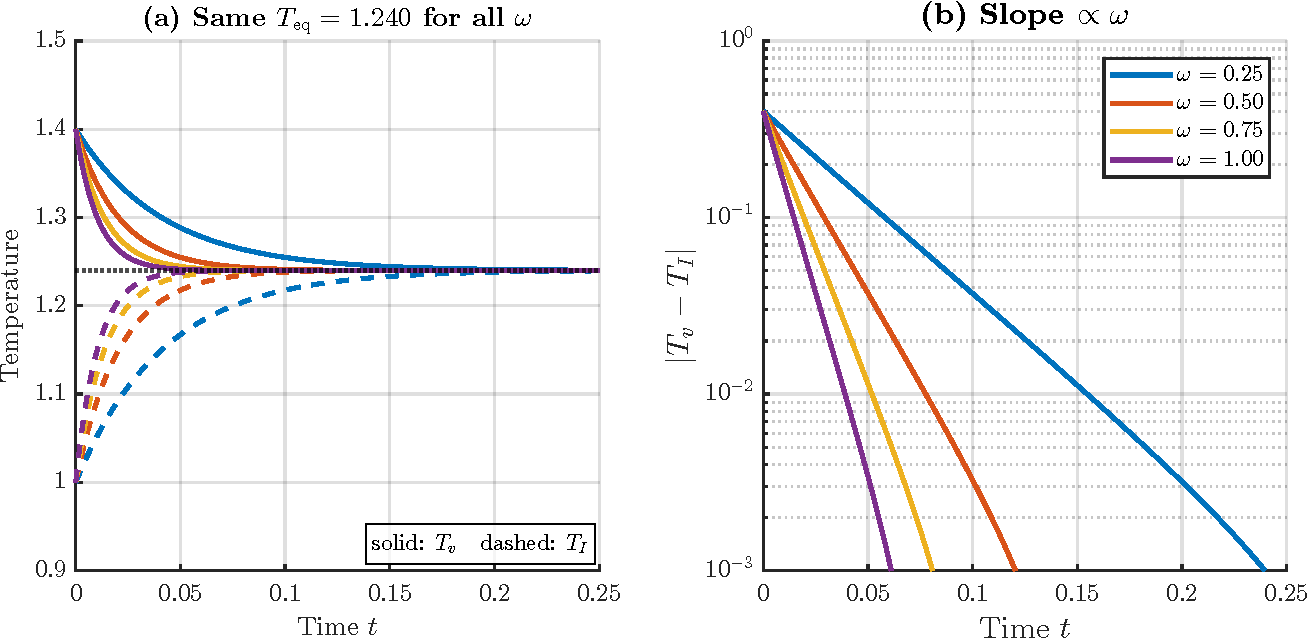
\includegraphics[width=0.9\textwidth]{figures/fig_polyrelax_sweep_omega.pdf}
\caption{Relaxation for varying DSMC weight $\omega$ at fixed $d_i=2$. (a) All $\omega$ reach the
same $T_{\mathrm{eq}}=1.240$. (b) The semilog decay of $|T_v-T_I|$ has slope proportional to
$\omega$ (measured rate $r$ in the legend), a direct consequence of the frozen channel being
elastic.}
\label{fig:relax_omega}
\end{figure}

\begin{figure}[t]
\centering
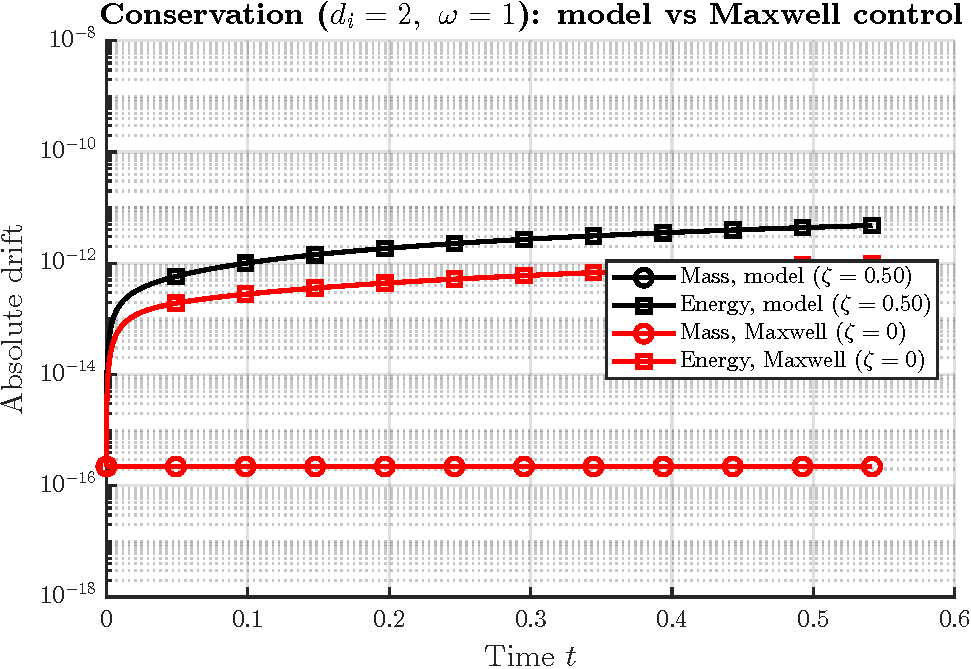
\includegraphics[width=0.62\textwidth]{figures/fig_polyrelax_conservation.pdf}
\caption{Conservation during the $d_i=2,\ \omega=1$ run. Total energy drifts by only
$\sim3\times10^{-12}$ (RK2 accumulation) and the mass row sits at the round-off floor, even though
$T_v$ and $T_I$ individually vary substantially.}
\label{fig:relax_cons}
\end{figure}
